
\documentclass{beamer}
\usepackage[british,spanish]{babel}
\usepackage[utf8]{inputenc}
\usepackage{hyperref}
\usepackage{multirow}



\usepackage{listings}

\usepackage{adjustbox}
\usepackage{lstcustom}

\usepackage{color}
\definecolor{light-gray}{gray}{0.80}
\definecolor{lstbackgroundshellcolor}{named}{light-gray}

\usepackage{tikz}
\newcommand*\circled[1]{\tikz[baseline=(char.base)]{
            \node[shape=circle,draw,inner sep=1pt] (char) {#1};}}

\usepackage[normalem]{ulem}

\newcommand{\outputcommand}[1]{\color{darkgreen}{#1|}}
\usepackage[acronym,xindy,toc]{glossaries}
\makeglossaries
%\usepackage[xindy]{imakeidx}
%\makeindex

\newcommand{\comment}[2]{#2}

\graphicspath{ {./images/} }

\title[Building a Scalable Architecture with Amazon SQS]{Building a Scalable Architecture with Amazon SQS}
%\subtitle[short subtitle]{long subtitle}
\author[C. Cuenca, F. Quintana]{Carmelo Cuenca-Hernández and Francisca Quintana-Domínguez}
%\institute{Escuela Universitaria de Informática}
%\date[04/2013]{Abril - 2013}
\date{}
\titlegraphic{
\includegraphics[width=0.5 \textwidth]{images/awslogo.eps}}



\pgfdeclareimage[width=2.0\baselineskip]{ulpgc-logo}{images/logosimbolo_secundario_version_vertical}
\setbeamertemplate{footline}{\raisebox{-2ex}{\pgfuseimage{ulpgc-logo}}
  \usebeamerfont{date in head/foot}\insertshortdate{}\hfill
  \usebeamertemplate{navigation symbols}\hfill
  \insertframenumber{}/\inserttotalframenumber}
\setbeamertemplate{sidebar right}{}


\usetheme{Antibes}
%\usetheme{Berlin}

%\usetheme{Warsaw}
%\usecolortheme{albatross}

\begin{document}

\begin{frame}
	\titlepage
\end{frame}


\section*{Outline}
\begin{frame}[fragile]
  \frametitle{Outline}
  %\tableofcontents%[part=1,pausesections]
  \tableofcontents[currentsection,currentsubsection, sectionstyle=show] 
  %\tableofcontents[currentsection,sectionstyle=show,hideothersubsections]
\end{frame}


\selectlanguage{british}

%%%%%%%%%%%%%%%%%%%%%%%%%%%%%%%%%%%%%%%%%%%%%%%%%%%%%%%%%%%%%%%%%%%%%%%%%%%%%%
%\newacronym{<label>}{<abbrv>}{<full>}
%\glsreset{<label>}
%\glsresetall
%\acrlong{<label>}
%\acrfull{<label>}
%\acrshort{<label>}
\newacronym{acl}{ACL}{Access Control List}
\newacronym{api}{API}{Application Programming Interface}
\newacronym{aws}{AWS}{Amazon Web Services}
\newacronym{cli}{CLI}{Command Line Interface}
\newacronym{css}{CSS}{cascading style sheets}
\newacronym{ebs}{EBS}{Elastic Block Storage}
\newacronym{ec2}{EC2}{Amazon Elastic Compute Cloud}
\newacronym{elb}{ELB}{Elastic Load Balancing}
\newacronym{iam}{IAM}{Identity Access Management}
\newacronym{ror}{RoR}{{\href{http://rubyonrails.org/}{Ruby on Rails}}}
\newacronym{rds}{RDS}{Relational Database Service}
\newacronym{rvm}{RVM}{{\href{https://rvm.io/}{Ruby Version Manager}}}
\newacronym{s3}{S3}{Simple Storage Service}
\newacronym{sqs}{SQS}{Amazon Simple Queue Service}


%%%%%%%%%%%%%%%%%%%%%%%%%%%%%%%%%%%%%%%%%%%%%%%%%%%%%%%%%%%%%%%%%%%%%%%%%%%%%
\section{Queue-Centric Workflow Pattern}
\begin{frame}[fragile,allowframebreaks]
\frametitle{Queue-Centric Workflow Pattern}
\begin{columns}
\column{0.6 \textwidth}
\begin{itemize}
\item The Queue-Centric Workflow Pattern is used in web aplications to decouple comunication between the web tier
(which implements the user interface) and the service tier (where business processing happens)
\end{itemize}
\column{0.4 \textwidth}
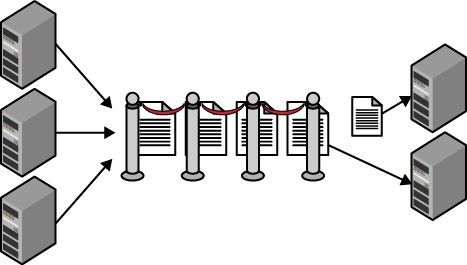
\includegraphics[width=0.75 \textwidth]{sqs.jpg}

\end{columns}
\end{frame}
%%%%%%%%%%%%%%%%%%%%%%%%%%%%%%%%%%%%%%%%%%%%%%%%%%%%%%%%%%%%%%%%%%%%%%%%%%%%%%

\section{Amazon Simple Queue Service}
\begin{frame}[fragile, allowframebreaks]
\frametitle{Amazon Simple Queue Service}
\begin{itemize}
\item \acrfull{sqs} is a fast, reliable, scalable, fully managed message queuing service. SQS makes it simple and cost-effective to decouple the components of a cloud application. You can use SQS to transmit any volume of data, at any level of throughput, without losing messages or requiring other services to be always available

\item With \acrshort{sqs}, you can offload the administrative burden of operating and scaling a highly available messaging cluster, while paying a low price for only what you use.

\item Service Highlights
\begin{itemize}
\item Reliable. Amazon \acrshort{sqs} runs within Amazon’s high-availability data centers, so queues will be available whenever applications need them. To prevent messages from being lost or becoming unavailable, all messages are stored redundantly across multiple servers and data centers
\item Scalable
\item Secure
\item Inexpensive
\end{itemize}

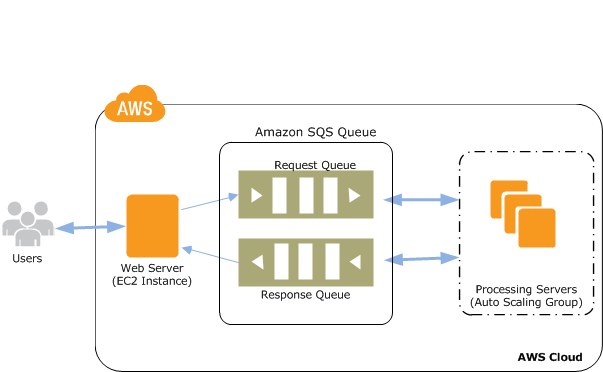
\includegraphics[width=0.75 \textwidth]{sqs-as-workflow.png}
\end{itemize}
\end{frame}
%%%%%%%%%%%%%%%%%%%%%%%%%%%%%%%%%%%%%%%%%%%%%%%%%%%%%%%%%%%%%%%%%%%%%%%%%%%%%
\begin{frame}[fragile, allowframebreaks]
\frametitle{Amazon SQS Overview}
\begin{itemize}
\item You can create any number of \acrshort{sqs} queues within the scope of your AWS account;
however, Amazon does reserve the right to delete queues if no messages have been
posted or retrieved for 30 consecutive days

\item Each queue has a name, which must be unique within a particular instance of \acrshort{sqs}
(there are currently instances of \acrshort{sqs} in the US and in Europe)
\item Every queue is identified by a unique queue URL. The URL is assigned when the
queue is created. All the operations on a queue require the specification of a queue
URL
\item Queues are used to store messages. Messages can be up to 8,192 bytes long. Due to
this low limit, messages should generally be used to pass pointers (for example,
URLs) to data stored elsewhere. Amazon \acrshort{s3} is often a good place to store data while
it’s being passed through a complex processing pipeline
certificate
\item Instead of being automatically deleted, a message retrieved from \acrshort{sqs} becomes
temporarily invisible so that it’s unable to be retrieved a second time. Once your
code retrieves a message, you have a certain amount of time—the visibility
timeout—to process and then delete the message. If the message is retained (or if
your application crashes while processing it), the message becomes visible once
again. This model allows you to build applications that avoid data loss as a result
of an application failure. The default value for the visibility timeout is 30 seconds
and the maximum value is 12 hours

\item When you retrieve a message from SQS, you also gain a receipt handle. You need
to hold on to this handle in order to delete the message after you’ve processed it.

\item Queues have a time limit: unprocessed messages will be silently deleted from the
queue after four days

\item You can choose to allow other applications and developers to access your queues
by using an access policy. The access policy gives you very granular control over
access to each aspect of SQS

\end{itemize}

\end{frame}
%%%%%%%%%%%%%%%%%%%%%%%%%%%%%%%%%%%%%%%%%%%%%%%%%%%%%%%%%%%%%%%%%%%%%%%%%%%%%
\begin{frame}[fragile, allowframebreaks]
\frametitle{Watch Out For \dots}
\begin{itemize}
\item \emph{Message Order}\\Because the queue is distributed, there’s no guarantee that SQS will return the
messages in the same order that they were sent. Your application logic must be
written so that it avoids relying on receiving messages in any particular order
\item \emph{Message Delivery}\\ Under very rare circumstances, SQS can return the same message more than
once. Your application can either treat messages as idempotent (so that pro-
cessing the same one more than once has no ill affect), or it can store a state
indicator in another location, such as Amazon SimpleDB.
\item \emph{Message Sampling}\\When your application asks SQS to return a message from a queue, SQS checks
a subset of the actual set of servers used to store the queue. If a queue contains
less than 1,000 items, the first retrieval may return no items but a second one
will
\end{itemize}
\end{frame}
%%%%%%%%%%%%%%%%%%%%%%%%%%%%%%%%%%%%%%%%%%%%%%%%%%%%%%%%%%%%%%%%%%%%%%%%%%%%%
\begin{frame}[fragile]
\frametitle{Operations}
As you’ll soon see, the SQS programming model is very simple. You can:
\begin{itemize}
\item create and delete queues from your account, and list your queues
\item send, receive, and delete messages, and change message attributes such as the
visibility timeout
\item control a queue’s access permissions on a very fine-grained basis
\end{itemize}
\end{frame}
%%%%%%%%%%%%%%%%%%%%%%%%%%%%%%%%%%%%%%%%%%%%%%%%%%%%%%%%%%%%%%%%%%%%%%%%%%%%%

\begin{frame}[fragile, allowframebreaks]
\frametitle{Pricing Model}
\begin{itemize}
\item \emph{Request}\\You pay \$0.01 (one cent) for every 10,000 SQS requests that you make. This is
equivalent to a price of \$0.000001 per request. Although the per-request price is very low, you still need to be careful
\item \emph{Data}\\Your data transfer charges are based on the amount of data transferred in and out
of SQS. Data transferred into SQS is charged at a rate of \$0.10 per gigabyte. Once
again, this amount is prorated. Data transferred out of SQS is charged on a sliding
scale starting at \$0.17 per gigabyte and decreasing with volume, reaching \$0.10 per
gigabyte for all outgoing data transfer in excess of 150 terabytes per month
\item There’s no charge for data transferred within a Region
\end{itemize}
\end{frame}
%%%%%%%%%%%%%%%%%%%%%%%%%%%%%%%%%%%%%%%%%%%%%%%%%%%%%%%%%%%%%%%%%%%%%%%%%%%%%
%%%%%%%%%%%%%%%%%%%%%%%%%%%%%%%%%%%%%%%%%%%%%%%%%%%%%%%%%%%%%%%%%%%%%%%%%%%%%
\section{Programming Amazon SQS}
%%%%%%%%%%%%%%%%%%%%%%%%%%%%%%%%%%%%%%%%%%%%%%%%%%%%%%%%%%%%%%%%%%%%%%%%%%%%%
\begin{frame}[fragile]
\frametitle{Programming Amazon SQS}
\begin{itemize}
\item Creating a Queue
\item Listing Queues
\item Inserting Items into Queues
\item Extracting Items from Queues
\end{itemize}
\end{frame}
%%%%%%%%%%%%%%%%%%%%%%%%%%%%%%%%%%%%%%%%%%%%%%%%%%%%%%%%%%%%%%%%%%%%%%%%%%%%%
%%%%%%%%%%%%%%%%%%%%%%%%%%%%%%%%%%%%%%%%%%%%%%%%%%%%%%%%%%%%%%%%%%%%%%%%%%%%%
\begin{frame}[fragile]
\frametitle{Creating Queues}
\lstset{language=Ruby, style=eclipse}
\begin{lstlisting}[escapechar=&]
#
# aws_app/sqs/create_queues.rb
#
# Usage: ruby create_queues.rb name1 [name2] ...
#
require File.expand_path(File.dirname(__FILE__) + '/../config')

abort "Usage: #{__FILE__} <QUEUE_NAME1> [QUEUE_NAME2] ..." unless ARGV.size != 0

# get an instance of the SQS interface using the default configuration
sqs = AWS::SQS.new

ARGV.each do |queue|
  sqs.queues.create queue
  puts "Created queue #{queue}"
end
\end{lstlisting}
\end{frame}
%%%%%%%%%%%%%%%%%%%%%%%%%%%%%%%%%%%%%%%%%%%%%%%%%%%%%%%%%%%%%%%%%%%%%%%%%%%%%
%%%%%%%%%%%%%%%%%%%%%%%%%%%%%%%%%%%%%%%%%%%%%%%%%%%%%%%%%%%%%%%%%%%%%%%%%%%%%
\begin{frame}[fragile]
\frametitle{Listing Queues}
\lstset{language=Ruby, style=eclipse}
\begin{lstlisting}[escapechar=&]
#
# aws_app/sqs/list_queues.rb
#
# Usage: ruby list_queues.rb
#
require File.expand_path(File.dirname(__FILE__) + '/../config')
	
# get an instance of the SQS interface using the default configuration
sqs = AWS::SQS.new
	
sqs.queues.each do |queue|
  puts queue.url
end
\end{lstlisting}

\lstset{language=shell}
\begin{lstlisting}[escapechar=!]
$ ruby sqs/list_queues.rb 
!\outputcommand{https://sqs.us-east-1.amazonaws.com/015850082106/c\_feed\\
https://sqs.us-east-1.amazonaws.com/015850082106/c\_image\\
https://sqs.us-east-1.amazonaws.com/015850082106/c\_parse\\
https://sqs.us-east-1.amazonaws.com/015850082106/c\_render\\
https://sqs.us-east-1.amazonaws.com/015850082106/c\_url}!
\end{lstlisting}
\end{frame}
%%%%%%%%%%%%%%%%%%%%%%%%%%%%%%%%%%%%%%%%%%%%%%%%%%%%%%%%%%%%%%%%%%%%%%%%%%%%%
%%%%%%%%%%%%%%%%%%%%%%%%%%%%%%%%%%%%%%%%%%%%%%%%%%%%%%%%%%%%%%%%%%%%%%%%%%%%%
\begin{frame}[fragile, allowframebreaks]
\frametitle{Inserting Items into Queues}
\lstset{language=Ruby, style=eclipse}
\begin{lstlisting}[escapechar=&]
#
# aws_app/sqs/post_queue.rb
#
# Usage: ruby post_queue.rb <QUEUE_NAME>  <MESSAGE1> ...
#
require File.expand_path(File.dirname(__FILE__) + '/../config')

(queue_name, *messages) = ARGVcertificate
abort "Usage: #{__FILE__}  <QUEUE_NAME>  <MESSAGE> ..." unless queue_name && messages.size != 0

# get an instance of the SQS interface using the default configuration
sqs = AWS::SQS.new
begin
  queue = sqs.queues.named queue_name
rescue
  abort "#{$!.class}: #{$!.message}"
end

messages.each do |message|
  queue.send_message message
  puts "Posted message #{message} to queue #{queue.url}"
end
\end{lstlisting}
\end{frame}
%%%%%%%%%%%%%%%%%%%%%%%%%%%%%%%%%%%%%%%%%%%%%%%%%%%%%%%%%%%%%%%%%%%%%%%%%%%%%
%%%%%%%%%%%%%%%%%%%%%%%%%%%%%%%%%%%%%%%%%%%%%%%%%%%%%%%%%%%%%%%%%%%%%%%%%%%%%
\begin{frame}[fragile, allowframebreaks]
\frametitle{Extracting Items from Queues}
\lstset{language=Ruby, style=eclipse}
\begin{lstlisting}[escapechar=&]
#
# aws_app/sqs/post_queue.rb
#
# Usage: ruby pull_queue.rb <QUEUE_NAME>
#
require File.expand_path(File.dirname(__FILE__) + '/../config')

abort "Usage: #{__FILE__} <QUEUE_NAME>" unless ARGV.size != 0

# get an instance of the SQS interface using the default configuration
sqs = AWS::SQS.new
queue_name = ARGV[0]
begin
  queue = sqs.queues.named queue_names
rescue
  abort "#{$!.class}: #{$!.message}"
end


#You can receive messages from the queue 
# (a) manually with the receive_message + delete_message, iterating while true
# (b) automatically, using poll that iterates, receive and delete the messages
#     In case (b) you can set the time to wait between receivings,...

#option (a)
=begin
while true
  queue.receive_message do |message|
    puts "Body message = #{message.body}"
    message.delete
  end
end
=end

# option (b)
queue.poll(:initial_timeout => false,
           :idle_timeout => 10) { |msg| puts msg.body }
\end{lstlisting}

\lstset{language=shell}
\begin{lstlisting}[escapechar=&]
$ ruby sqs/create_queue perdidita
$ ruby sqs/post_queue.rb perdidita 'Hello World!"
$ ruby sqs/pull_queue.rb perdiditacertificate
&\outputcommand{\\
be patient \dots\\
Hello World!
}&
\end{lstlisting}
\end{frame}
%%%%%%%%%%%%%%%%%%%%%%%%%%%%%%%%%%%%%%%%%%%%%%%%%%%%%%%%%%%%%%%%%%%%%%%%%%%%%
\section{Building a Image Crawler}
%%%%%%%%%%%%%%%%%%%%%%%%%%%%%%%%%%%%%%%%%%%%%%%%%%%%%%%%%%%%%%%%%%%%%%%%%%%%%
\begin{frame}[fragile, allowframebreaks]
\frametitle{Building a Image Crawler}

\begin{center}
 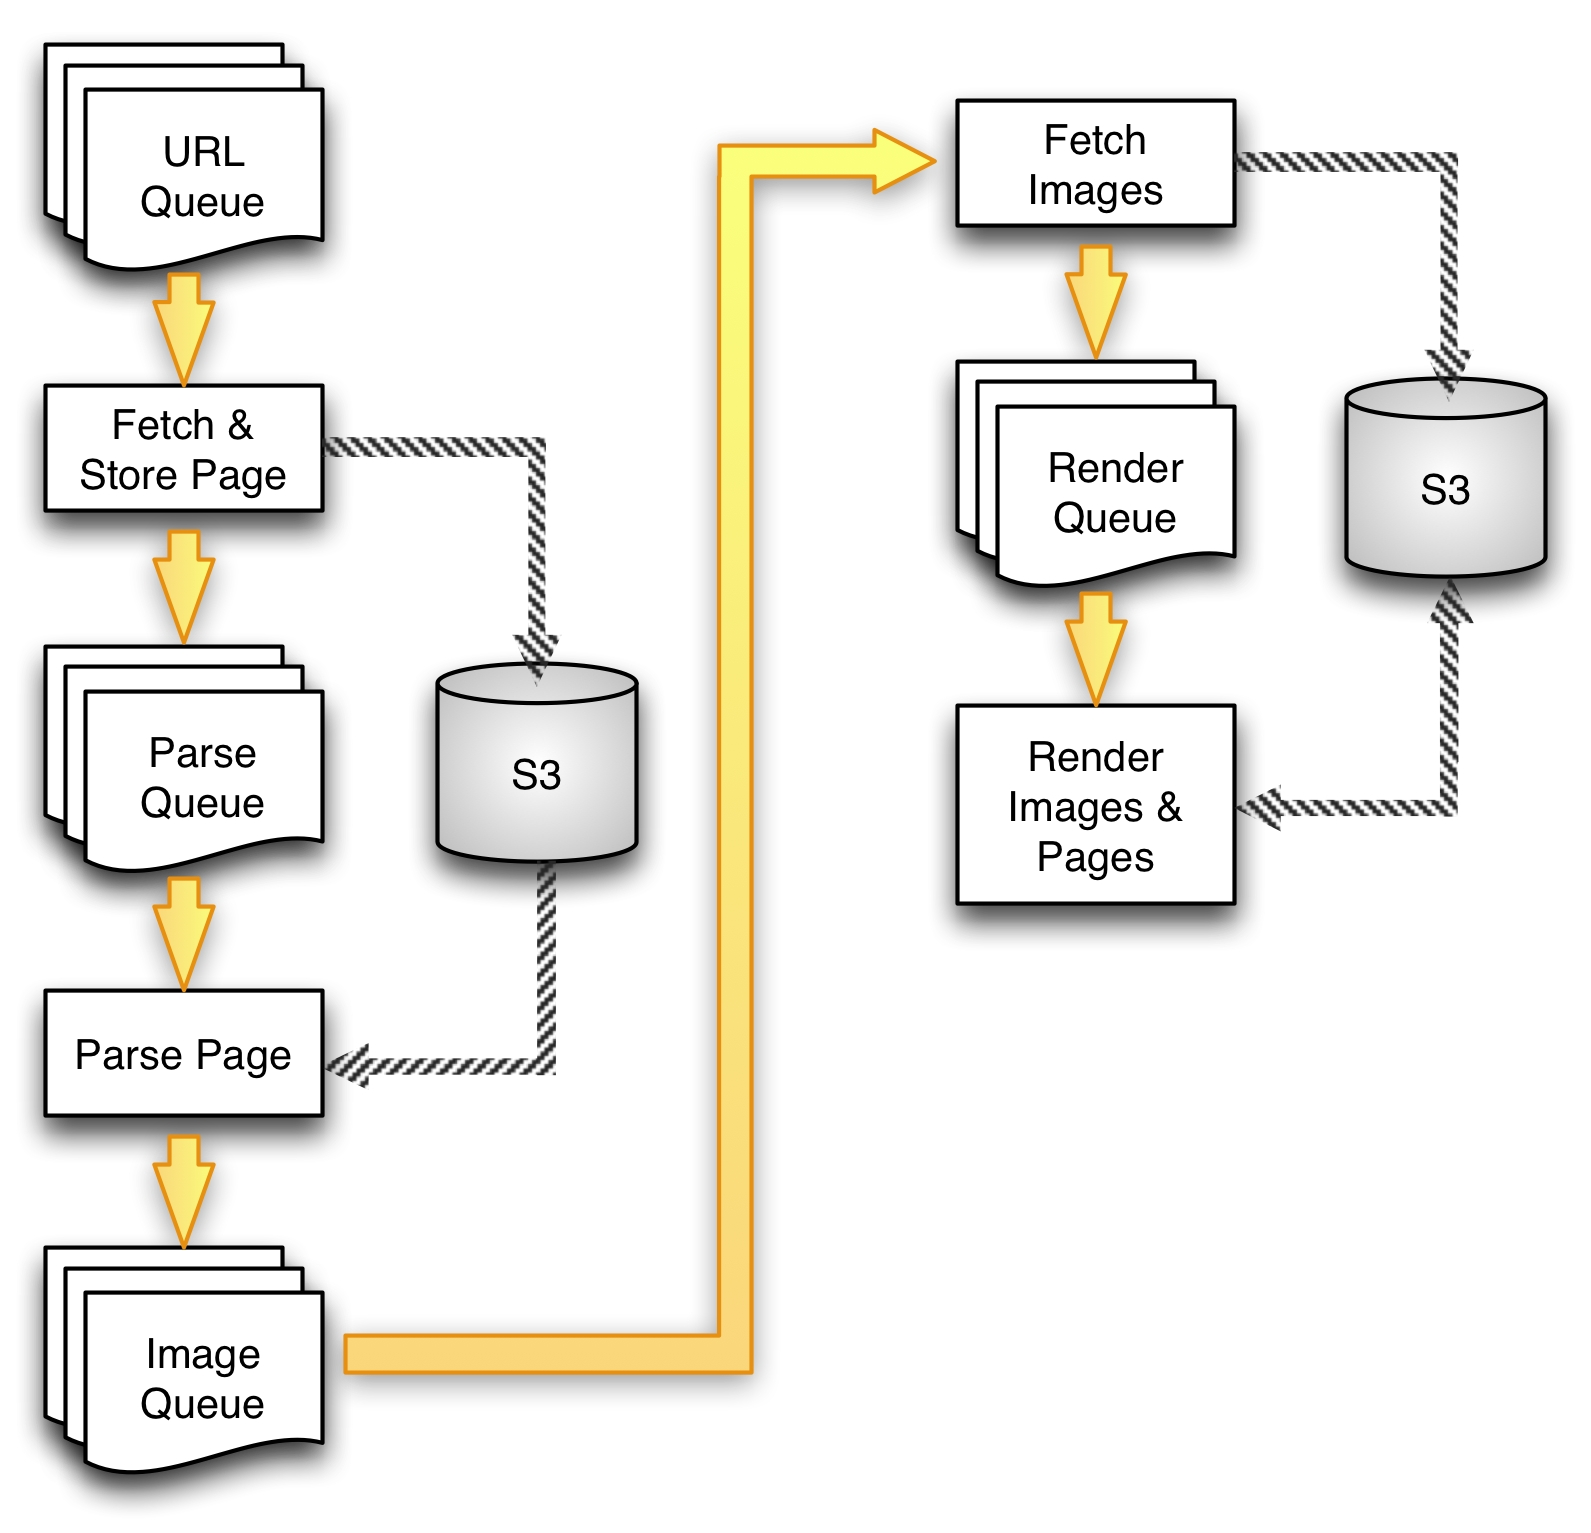
\includegraphics[ width= 0.5 \textwidth]{image-crawler.jpg}
\end{center}


\begin{itemize}
\item The application will be an image crawler:
\begin{enumerate}
\item Given the URL of a web page, the crawler
will download the page and store it in Amazon S3
\item It will then parse the page, looking for HTML image tags, downloading all the images on the page to S3, and
scaling them to a common size
\item After all the images on the page have been downloaded, they’ll be used to draw a single, composite image. The composite image
will contain all the scaled images from the original page.
\end{enumerate}
\end{itemize}

\lstset{language=shell}
\begin{lstlisting}[escapechar=&]
$ ruby sqs/create_queue perdidita
$ ruby sqs/post_queue.rb perdidita 'Hello World!"
$ ruby sqs/pull_queue.rb perdiditacertificate
&\outputcommand{\\
be patient \dots\\
Hello World!
}&
\end{lstlisting}

\end{frame}
%%%%%%%%%%%%%%%%%%%%%%%%%%%%%%%%%%%%%%%%%%%%%%%%%%%%%%%%%%%%%%%%%%%%%%%%%%%%%
%%%%%%%%%%%%%%%%%%%%%%%%%%%%%%%%%%%%%%%%%%%%%%%%%%%%%%%%%%%%%%%%%%%%%%%%%%%%%
\begin{frame}[fragile, allowframebreaks]
\frametitle{Definitions and Utility Functions}

\lstset{language=Ruby, style=eclipse}

\begin{itemize}
\item Because each queue will be referenced by several processes, let’s define some symbolic names for them in a new  book.inc.php file:

\begin{lstlisting}[escapechar=&]
#
# aws_app/crawler/book.inc.rb
#
# This file define constant to crawler application

URL_QUEUE = 'c_url'
PARSE_QUEUE = 'c_parse'
IMAGE_QUEUE = 'c_image'
RENDER_QUEUE = 'c_render'
\end{lstlisting}

\end{itemize}


\end{frame}
%%%%%%%%%%%%%%%%%%%%%%%%%%%%%%%%%%%%%%%%%%%%%%%%%%%%%%%%%%%%%%%%%%%%%%%%%%%%%
%%%%%%%%%%%%%%%%%%%%%%%%%%%%%%%%%%%%%%%%%%%%%%%%%%%%%%%%%%%%%%%%%%%%%%%%%%%%%
\begin{frame}[fragile, allowframebreaks]
\frametitle{Crawl Loader Command}

\begin{itemize}
\item We need a way to load a URL into the first stage of the pipeline. Here’s a command
line tool to do just that:
\lstset{language=Ruby, style=eclipse}
\begin{lstlisting}
#
# aws_app/crawler/load_crawl_urls.rb
#

require File.expand_path("#{File.dirname(__FILE__)}/../config")
require File.expand_path("#{File.dirname(__FILE__)}/book.inc")

abort "Usage: #{__FILE__} <URL(s)>" unless ARGV.size != 0

# get an instance of the SQS interface using the default configuration
sqs = AWS::SQS.new

# get the queue whose name is URL_QUEUE
begin
  queue = sqs.queues.named URL_QUEUE
rescue
  abort "#{$!.class}: #{$!.message}"
end

# for each url in the command line, build the message, encode it to JSON,
# send it to queue c_url
ARGV.each do |url|
  message = {action: 'Fetchpage',
             origin: __FILE__,
             data: url,
             history: "Posted by #{__FILE__} at #{Time.now}"}.to_json
  begin
    queue.send_message message
    puts "Posted message #{message} to queue #{queue.url}"
  rescue
    puts "#{$!.class}: #{$!.message}"
  end
end
\end{lstlisting}


\item The URL and some additional information are bundled as an array. We then call
the json\_encode function to convert the array into a JSON value (the message
stored in the variable \texttt{message}) and the send\_message method to post it to the
\texttt{URL\_QUEUE queue}

\item Here’s how to use this tool:
\lstset{language=shell}
\begin{lstlisting}[escapechar=!]
$ ruby crawler/load\_crawl\_urls.rb http://www.freedigitalphotos.net/images/People\_g40.html http://www.sxc.hu/category/115 http://www.stockfreeimages.com/c1/it-c/connectivity.html http://www.turbophoto.com/Sports.html
!\outputcommand{Posted message \{"action":"Fetchpage","origin":"crawler/load\_crawl\_urls.rb","data":"http://www.freedigitalphotos.net/images/People\_g40.html","history":"Posted by crawler/load\_crawl\_urls.rb at 2014-02-24 10:47:22 +0000"\} to queue https://sqs.us-east-1.amazonaws.com/015850082106/c\_url\\
\dots}!
\end{lstlisting}

\end{itemize}


\end{frame}
%%%%%%%%%%%%%%%%%%%%%%%%%%%%%%%%%%%%%%%%%%%%%%%%%%%%%%%%%%%%%%%%%%%%%%%%%%%%%
%%%%%%%%%%%%%%%%%%%%%%%%%%%%%%%%%%%%%%%%%%%%%%%%%%%%%%%%%%%%%%%%%%%%%%%%%%%%%
\begin{frame}[fragile]
\frametitle{The Feed Processing Pipeline}
\begin{itemize}
\item Now we have the tools needed to implement the four stages of our processing
pipeline:
\begin{enumerate}
\item fetch the HTML
\item parse the HTML and extract the image URLs
\item fetch the images and create thumbnails
\item render the final mosaic image
\end{enumerate}
\end{itemize}
\end{frame}
%%%%%%%%%%%%%%%%%%%%%%%%%%%%%%%%%%%%%%%%%%%%%%%%%%%%%%%%%%%%%%%%%%%%%%%%%%%%%
\begin{frame}[fragile, allowframebreaks]
\frametitle{Stage 1 - Fetching the HTML}

\begin{itemize}
 \item This stage is fairly simple. It pulls a URL from the \texttt{URL\_QUEUE} queue and fetches the
HTML at the URL. It stores the HTML in Amazon S3 and then passes the work along
to the next stage in the pipeline by writing a message to the \texttt{PARSE\_QUEUE} queue
\lstset{language=Ruby, style=eclipse}
\begin{lstlisting}[escapechar=&]
#
# aws_app/crawler/fetch_page.rb
#

require 'net/http'
require File.expand_path(File.dirname(__FILE__) + '/../config')
require File.expand_path(File.dirname(__FILE__) + '/book.inc')
require File.expand_path("#{File.dirname(__FILE__)}/../s3/book.inc")

# get an instance of the SQS and S3 interfaces using the default configuration
sqs = AWS::SQS.new
s3 = AWS::S3.new

begin
  sqs.queues.create URL_QUEUE
  queue_in = sqs.queues.named URL_QUEUE
  sqs.queues.create PARSE_QUEUE
  queue_out = sqs.queues.named PARSE_QUEUE
rescue
  abort "#{$!.class}: #{$!.message}"
end

bucket = s3.buckets.create BOOK_BUCKET
abort "Error creating #{bucket_name} bucket" unless bucket.exists?

# Receive messages from the url queue (forever loop)
queue_in.poll do |msg|
  page_url = JSON.parse(msg.body)['data']  # &\circled{1}&
  puts "Processing URL: #{page_url}"
  web_contents  = Net::HTTP.get(URI.parse(page_url))  # &\circled{2}&
  puts "Retrieved #{web_contents.length} bytes of HTML"
  key = 'page_' + Digest::MD5.hexdigest(page_url) + '.html' # &\circled{3}&
  if upload_object( s3, bucket, key, web_contents, 'text/html' )
    puts "Uploaded page to S3 as #{key}"

    message = {action: 'ParsePage',
               origin: __FILE__,
               page_url: page_url,
               data: "http://s3.amazonaws.com/#{BOOK_BUCKET}/#{key}",
               history: "Posted by #{__FILE__} at #{Time.now}"}.to_json # &\circled{1}&
    begin
      queue_out.send_message message
      puts "Posted message #{message} to queue #{queue_out.url}"
    rescue
      puts "#{$!.class}: #{$!.message}"
    end
  else
    puts 'Error uploading HTML to S3'
  end
end
\end{lstlisting}

\item Here’s how to use this tool:
\lstset{language=shell}
\begin{lstlisting}[escapechar=!]
$ ruby crawler/fetch_page.rb
!\outputcommand{
Processing URL: http://www.sxc.hu/category/115\\
Retrieved 42550 bytes of HTML\\
Uploaded page to S3 as page\_bb06539925ead884f75663edbccecba5.html\\
Posted message\\ {"action":"ParsePage","origin":"crawler/fetch\_page.rb","page\_url":"http://www.sxc.hu/category/115","data":"http://s3.amazonaws.com/developing\_cloud\_application\_bucket/page\_bb06539925ead884f75663edbccecba5.html","history":"Posted by crawler/fetch\_page.rb at 2014-02-24 12:21:56 +0000"} to queue\\ https://sqs.us-east-1.amazonaws.com/015850082106/c\_parse\\
!\dots!}
\end{lstlisting}
\end{itemize}
\end{frame}
%%%%%%%%%%%%%%%%%%%%%%%%%%%%%%%%%%%%%%%%%%%%%%%%%%%%%%%%%%%%%%%%%%%%%%%%%%%%%
\begin{frame}[fragile, allowframebreaks]
\frametitle{Stage 2 - Parsing HTML and Extracting Image URLs}
\begin{itemize}
\item This stage pulls the raw HTML from
S3, parses it using a third-party HTML parser, extracts some of the image links, and
passes those links on to the next stage
\item To simplify this example, we’ll only process images that have an relative URL
\lstset{language=Ruby, style=eclipse}
\begin{lstlisting}[escapechar=&]
#
# aws_app/crawler/parse_page.rb
#

require 'nokogiri'
require 'open-uri'

require File.expand_path(File.dirname(__FILE__) + '/../config')
require File.expand_path(File.dirname(__FILE__) + '/book.inc')

# get an instance of the SQS using the default configuration
sqs = AWS::SQS.new

begin
  sqs.queues.create PARSE_QUEUE
  queue_in = sqs.queues.named PARSE_QUEUE
  sqs.queues.create IMAGE_QUEUE
  queue_out = sqs.queues.named IMAGE_QUEUE
rescue
  abort "#{$!.class}: #{$!.message}"
end

# Receive messages from the parse queue (forever loop)
queue_in.poll do |msg|
  s3_page_url = JSON.parse(msg.body)['data']
  page_url = JSON.parse(msg.body)['page_url']

  puts "Processing URL: #{s3_page_url} with original #{page_url}"

  img_urls = []
  doc = Nokogiri::HTML(open(s3_page_url).read)
  doc.css('//img/@src').each do |link|  # &\circled{1}&
    # catching images with relative paths and building the full path
    img_urls << URI.escape(URI.parse(page_url).scheme + '://' + URI.parse(page_url).host + '/' + link.content)  # &\circled{2}&
  end
  puts "Processing image #{img_urls}"
  if img_urls.length != 0
    message = {action: 'FetchImages',
               origin: __FILE__,
               data: img_urls,
               history: "Posted by #{__FILE__} at #{Time.now}",
               title: doc.css('title').text}.to_json
    begin
      queue_out.send_message message  # &\circled{3}&
      puts "Posted message #{message} to queue #{queue_out.url}"
    rescue
      puts "#{$!.class}: #{$!.message}"
    end
  end
end

\end{lstlisting}

\item Here’s how to use this tool:
\lstset{language=shell}
\begin{lstlisting}[escapechar=&]
$ ruby crawler/parse_page.rb 
&\outputcommand{Processing URL: http://s3.amazonaws.com/developing\_cloud\_application\_bucket/page\_a1690b0f6347aadb4d700c627c8fe3a8.html with original http://www.freedigitalphotos.net/images/People\_g40.html\\
Processing image ["http://www.freedigitalphotos.net/images/cart.png", "http://www.freedigitalphotos.net/images/nav\_arrow.gif",\\ "http://www.freedigitalphotos.net/gal\_images/av-\_146.jpg", "http://www.freedigitalphotos.net/gal\_images/av-\_332.jpg"\\
\dots}&
\end{lstlisting}

\end{itemize}
\end{frame}
%%%%%%%%%%%%%%%%%%%%%%%%%%%%%%%%%%%%%%%%%%%%%%%%%%%%%%%%%%%%%%%%%%%%%%%%%%%%%
\begin{frame}[fragile, allowframebreaks]
\frametitle{Stage 3 - Fetching Image URLs}
\begin{itemize}
\item This stage takes the array of image URLs from the previous stage, and fetches each
one. It then uses the \texttt{thumbnail\_image} function that we wrote  to scale
the image to a smaller size, as defined by the \texttt{THUMB\_SIZE} constant
\lstset{language=Ruby, style=eclipse}
\begin{lstlisting}[escapechar=&]
#
# aws_app/crawler/fetch_images.rb
#

require 'net/http'
require File.expand_path(File.dirname(__FILE__) + '/../config')
require File.expand_path(File.dirname(__FILE__) + '/book.inc')
require File.expand_path(File.dirname(__FILE__) + '/../s3/book.inc')

# get an instance of the SQS and S3 interfaces using the default configuration
sqs = AWS::SQS.new
s3 = AWS::S3.new

begin
  sqs.queues.create IMAGE_QUEUE
  queue_in = sqs.queues.named IMAGE_QUEUE
  sqs.queues.create RENDER_QUEUE
  queue_out = sqs.queues.named RENDER_QUEUE
rescue
  abort "#{$!.class}: #{$!.message}"
end

bucket = s3.buckets.create BOOK_BUCKET
abort "Error creating #{bucket_name} bucket" unless bucket.exists?

# Receive messages from the url queue (forever loop)
queue_in.poll do |msg|
  s3_image_keys = []

  puts " Retrieved message: Image URLs: #{JSON.parse(msg.body)['data']}"
  JSON.parse(msg.body)['data'].each do |img_url|
    puts "Processing image: #{img_url}"
    img_contents  = Net::HTTP.get(URI.parse(img_url))  # &\circled{1} &
    puts "Retrieved #{img_contents.length} bytes of image"
    begin
      img_out = thumbnail_image img_contents  # &\circled{2} &
      puts 'Generated thumbnail'
      key = "image_#{Digest::MD5.hexdigest(img_url)}.png"

      if upload_object( s3, bucket, key, img_out, 'image/png' )   # &\circled{3} &
        puts "Uploaded image to S3 as #{key}"
        s3_image_keys << key
      else
        puts "Error uploading image #{img_url} to S3"
      end
      break if s3_image_keys.size >= 16
    rescue
      puts "#{$!.class}: #{$!.message}"
    end

  end

  if s3_image_keys.size > 0   # &\circled{4} &
    message = {action: 'RenderPage',
               origin: __FILE__,
               data: s3_image_keys,
               history: "Posted by #{__FILE__} at #{Time.now}",
               page_title: JSON.parse(msg.body)['title']}.to_json
    begin
      queue_out.send_message message
      puts "Posted message #{message} to queue #{queue_out.url}"
    rescue
      puts "#{$!.class}: #{$!.message}"
    end
  end
end
\end{lstlisting}
\item Here’s how to use this tool:
\lstset{language=shell}
\begin{lstlisting}
$ ruby crawler/fetch_images.rb 
\end{lstlisting}
\end{itemize}
\end{frame}
%%%%%%%%%%%%%%%%%%%%%%%%%%%%%%%%%%%%%%%%%%%%%%%%%%%%%%%%%%%%%%%%%%%%%%%%%%%%%
%%%%%%%%%%%%%%%%%%%%%%%%%%%%%%%%%%%%%%%%%%%%%%%%%%%%%%%%%%%%%%%%%%%%%%%%%%%%%
\begin{frame}[fragile, allowframebreaks]
\frametitle{Stage 4 - Render Images}
\begin{itemize}
\item The fourth and final stage takes the S3 object keys and fetches each object from S3
before generating a thumbnail mosaic image

\lstset{language=Ruby, style=eclipse}
\begin{lstlisting}[escapechar=&]
#
# aws_app/crawler/render_image.rb
#
require File.expand_path(File.dirname(__FILE__) + '/../config')
require File.expand_path(File.dirname(__FILE__) + '/book.inc')
require File.expand_path("#{File.dirname(__FILE__)}/../s3/book.inc")

def new_image(width, height, format = "png", bgcolor = "transparent")
  tmp = Tempfile.new(%W[mini_magick_ .#{format}])
  `convert -size #{width}x#{height} xc:#{bgcolor} #{tmp.path}`
  MiniMagick::Image.new(tmp.path, tmp)
end

# get an instance of the SQS and S3 interfaces using the default configuration
sqs = AWS::SQS.new
s3 = AWS::S3.new

begin
  sqs.queues.create RENDER_QUEUE
  queue_in = sqs.queues.named RENDER_QUEUE
rescue
  abort "#{$!.class}: #{$!.message}"
end

bucket = s3.buckets.create BOOK_BUCKET
abort "Error creating #{bucket_name} bucket" unless bucket.exists?

# Receive messages from the render queue (forever loop)

s3_image_keys = []
queue_in.poll do |msg|
  x_offset = 0
  y_offset = 0
  image_array = JSON.parse(msg.body)['data']
  width = Integer(Math.sqrt  image_array.length)
  output_image = new_image width*THUMB_SIZE, width*THUMB_SIZE , 'png', 'transparent'

  image_array.each do |img_url|
    puts "image_location = http://s3.amazonaws.com/#{BOOK_BUCKET}/#{img_url}"
    tmp_image = MiniMagick::Image.open("http://s3.amazonaws.com/#{BOOK_BUCKET}/#{img_url}")
    output_image = output_image.composite(tmp_image,'png') do |c|
      c.gravity 'NorthWest'
      c.geometry "+#{x_offset*THUMB_SIZE}+#{y_offset*THUMB_SIZE}"
    end
    if (x_offset += 1) >= width
      x_offset, y_offset = 0 , y_offset + 1
    end
  end

  output_image_name = "#{JSON.parse(msg.body)['page_title']}.#{Time.now}.png"
  key = 'final_image_' + Digest::MD5.hexdigest(output_image_name) + '.png'
  if upload_object( s3, bucket, key, output_image.to_blob, 'image/png')
    p "Stored final image in S3 using key #{key}. URL:http://s3.amazonaws.com/#{BOOK_BUCKET}/#{key}"
  else
    puts "Error uploading image #{img_url} to S3"
  end
end
\end{lstlisting}
\item Here’s how to use this tool:
\lstset{language=shell}
\begin{lstlisting}[escapechar=!]
$ ruby crawler/render_image.rb 
!\outputcommand{image\_location = http://s3.amazonaws.com/developing\_cloud\_application\_bucket/image\_bfd43e28e9c24b6aa58be89ca9ddf2c1.png\\
image\_location = http://s3.amazonaws.com/developing\_cloud\_application\_bucket/image\_f65b5f3577de03898c83e8d56df44d0a.png\\
\dots\\
"Stored final image in S3 using key final\_image\_d6fe8533d597552e2858a793abd937e8.png. URL:http://s3.amazonaws.com/developing\_cloud\_application\_bucket/final\_image\_d6fe8533d597552e2858a793abd937e8.png"}!
\end{lstlisting}

\item You can run all proccess together writting \texttt{fetch\_page \&; parse\_page \&; fetch\_image \&; render\_image \& } and then run \texttt{load\_crawl\_url \dots} to start filling the first queue
\end{itemize}

\end{frame}
%%%%%%%%%%%%%%%%%%%%%%%%%%%%%%%%%%%%%%%%%%%%%%%%%%%%%%%%%%%%%%%%%%%%%%%%%%%%%
%%%%%%%%%%%%%%%%%%%%%%%%%%%%%%%%%%%%%%%%%%%%%%%%%%%%%%%%%%%%%%%%%%%%%%%%%%%%%
\section{Homework}
%%%%%%%%%%%%%%%%%%%%%%%%%%%%%%%%%%%%%%%%%%%%%%%%%%%%%%%%%%%%%%%%%%%%%%%%%%%%%
\begin{frame}[fragile]
\frametitle{Homework}
\begin{itemize}
\item ???
\end{itemize}
\end{frame}
%%%%%%%%%%%%%%%%%%%%%%%%%%%%%%%%%%%%%%%%%%%%%%%%%%%%%%%%%%%%%%%%%%%%%%%%%%%%%
\end{document}

\section*{Acronyms}
\begin{frame}
\frametitle[Acronyms]{Acronyms}
\glsaddall
\printglossary[type=\acronymtype] % prints just the list of acronyms
\end{frame}
%%%%%%%%%%%%%%%%%%%%%%%%%%%%%%%%%%%%%%%%%%%%%%%%%%%%%%%%%%%%%%%%%%%%%%%%%%%%%%
%%%%%%%%%%%%%%%%%%%%%%%%%%%%%%%%%%%%%%%%%%%%%%%%%%%%%%%%%%%%%%%%%%%%%%%%%%%%%%




